\documentclass[10pt]{beamer}

\usetheme{metropolis}
\usepackage{appendixnumberbeamer}
\usepackage[spanish]{babel}
\usepackage[utf8]{inputenc}
\usepackage[TS1,T1]{fontenc}
\usepackage{array}
\usepackage{graphicx}
\usepackage{colortbl}
\usepackage{caption}
\usepackage{subcaption}

\newcommand{\foo}{\color{gray}\makebox[0pt]{\textbullet}\hskip-0.5pt\vrule width 1pt\hspace{\labelsep}}

\usepackage{booktabs}
\usepackage[scale=2]{ccicons}

\usepackage{pgfplots}
\usepgfplotslibrary{dateplot}

\usepackage{multicol}

\usepackage{xspace}
\newcommand{\themename}{\textbf{\textsc{metropolis}}\xspace}

\title{Historia de los algoritmos inspirados en la evolución}
\subtitle{Algoritmos genéticos, programación evolutiva, estrategias de evolución y programación genética}
\date{\today}
\author{
  Francisco Luque Sánchez \\
  Ignacio Mas Mesa \\
  Miguel Morales Castillo \\
  María del Mar Ruiz Martín
}
\institute{Universidad de Granada}
% \titlegraphic{\hfill
\includegraphics[height=1.5cm]{logo.pdf}}

\begin{document}

\maketitle

\begin{frame}{Índice}
  \setbeamertemplate{section in toc}[sections numbered]
  \tableofcontents[hideallsubsections]
\end{frame}

\section{Introducción}

\begin{frame}[fragile]{Metaheurísticas}
  \begin{itemize}
  \item Aparecen en los años 50 (Optimización estocástica por Robbins y Monro) \\
  \item Resuelven problemas de optimización y búsqueda \\
  \item Tienen inspiraciones en procesos naturales \\
  \item Nos centraremos en las inspiradas en la evolución
  \end{itemize}
\end{frame}

\section{Programación evolutiva}

\begin{frame}[fragile]{Programación evolutiva}
  \begin{multicols}{2}
    ~\\
    \begin{itemize}
    \item Aparecen en 1964
    \item Su inventor es Lawrence J. Fogel
    \item Las utiliza para la predicción de series temporales
    \end{itemize}
    ~\\
    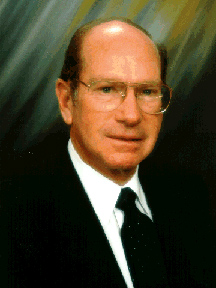
\includegraphics[scale=.6]{imgs/Fogel}
  \end{multicols}
\end{frame}

\begin{frame}{Primera propuesta}
  \begin{itemize}
  \item Representación de la línea temporal como cadena de símbolos
  \item Conjunto de autómatas finitos
  \item Evaluación de la capacidad de predicción
  \item Mutación de los autómatas (creación de la prole)
  \item Competición por la supervivencia (sobreviven los más aptos)
  \end{itemize}
\end{frame}

\begin{frame}{Evolución de la estrategia}
  \begin{table}
    \renewcommand\arraystretch{1.4}\arrayrulecolor{lightgray}
    \begin{tabular}{@{\,}r <{\hskip 2pt} !{\foo} >{\raggedright\arraybackslash}p{8cm}}
      \addlinespace[1.5ex]
      1969 & Aplicación a programas que juegan a juegos (Huntsinger)\\
      1980 & Nuevas representaciones de la solución (Fogel)\\
      1988 & Planificación de rutas (Fogel)\\
      1989 & Problema de la mochila (Fogel)\\
      1990 & Esquemas de adaptación de la evolución\\
      1992 & Aplicaciones en robótica (Donnel y Andersen)\\
      1995 & Diversificación del uso. Aplicación al entrenamiento de redes neuronales\\
    \end{tabular}
  \end{table}
\end{frame}

\section{Algoritmos genéticos}

\begin{frame}[fragile]{Typography}
      \begin{verbatim}The theme provides sensible defaults to
\emph{emphasize} text, \alert{accent} parts
or show \textbf{bold} results.\end{verbatim}

  \begin{center}becomes\end{center}

  The theme provides sensible defaults to \emph{emphasize} text,
  \alert{accent} parts or show \textbf{bold} results.
\end{frame}

\begin{frame}{Font feature test}
  \begin{itemize}
    \item Regular
    \item \textit{Italic}
    \item \textsc{SmallCaps}
    \item \textbf{Bold}
    \item \textbf{\textit{Bold Italic}}
    \item \textbf{\textsc{Bold SmallCaps}}
    \item \texttt{Monospace}
    \item \texttt{\textit{Monospace Italic}}
    \item \texttt{\textbf{Monospace Bold}}
    \item \texttt{\textbf{\textit{Monospace Bold Italic}}}
  \end{itemize}
\end{frame}

\begin{frame}{Lists}
  \begin{columns}[T,onlytextwidth]
    \column{0.33\textwidth}
      Items
      \begin{itemize}
        \item Milk \item Eggs \item Potatos
      \end{itemize}

    \column{0.33\textwidth}
      Enumerations
      \begin{enumerate}
        \item First, \item Second and \item Last.
      \end{enumerate}

    \column{0.33\textwidth}
      Descriptions
      \begin{description}
        \item[PowerPoint] Meeh. \item[Beamer] Yeeeha.
      \end{description}
  \end{columns}
\end{frame}
\begin{frame}{Animation}
  \begin{itemize}[<+- | alert@+>]
    \item \alert<4>{This is\only<4>{ really} important}
    \item Now this
    \item And now this
  \end{itemize}
\end{frame}
\begin{frame}{Figures}
  \begin{figure}
    \newcounter{density}
    \setcounter{density}{20}
    \begin{tikzpicture}
      \def\couleur{alerted text.fg}
      \path[coordinate] (0,0)  coordinate(A)
                  ++( 90:5cm) coordinate(B)
                  ++(0:5cm) coordinate(C)
                  ++(-90:5cm) coordinate(D);
      \draw[fill=\couleur!\thedensity] (A) -- (B) -- (C) --(D) -- cycle;
      \foreach \x in {1,...,40}{%
          \pgfmathsetcounter{density}{\thedensity+20}
          \setcounter{density}{\thedensity}
          \path[coordinate] coordinate(X) at (A){};
          \path[coordinate] (A) -- (B) coordinate[pos=.10](A)
                              -- (C) coordinate[pos=.10](B)
                              -- (D) coordinate[pos=.10](C)
                              -- (X) coordinate[pos=.10](D);
          \draw[fill=\couleur!\thedensity] (A)--(B)--(C)-- (D) -- cycle;
      }
    \end{tikzpicture}
    \caption{Rotated square from
    \href{http://www.texample.net/tikz/examples/rotated-polygons/}{texample.net}.}
  \end{figure}
\end{frame}
\begin{frame}{Tables}
  \begin{table}
    \caption{Largest cities in the world (source: Wikipedia)}
    \begin{tabular}{lr}
      \toprule
      City & Population\\
      \midrule
      Mexico City & 20,116,842\\
      Shanghai & 19,210,000\\
      Peking & 15,796,450\\
      Istanbul & 14,160,467\\
      \bottomrule
    \end{tabular}
  \end{table}
\end{frame}
\begin{frame}{Blocks}
  Three different block environments are pre-defined and may be styled with an
  optional background color.

  \begin{columns}[T,onlytextwidth]
    \column{0.5\textwidth}
      \begin{block}{Default}
        Block content.
      \end{block}

      \begin{alertblock}{Alert}
        Block content.
      \end{alertblock}

      \begin{exampleblock}{Example}
        Block content.
      \end{exampleblock}

    \column{0.5\textwidth}

      \metroset{block=fill}

      \begin{block}{Default}
        Block content.
      \end{block}

      \begin{alertblock}{Alert}
        Block content.
      \end{alertblock}

      \begin{exampleblock}{Example}
        Block content.
      \end{exampleblock}

  \end{columns}
\end{frame}
\begin{frame}{Math}
  \begin{equation*}
    e = \lim_{n\to \infty} \left(1 + \frac{1}{n}\right)^n
  \end{equation*}
\end{frame}
\begin{frame}{Line plots}
  \begin{figure}
    \begin{tikzpicture}
      \begin{axis}[
        mlineplot,
        width=0.9\textwidth,
        height=6cm,
      ]

        \addplot {sin(deg(x))};
        \addplot+[samples=100] {sin(deg(2*x))};

      \end{axis}
    \end{tikzpicture}
  \end{figure}
\end{frame}
\begin{frame}{Bar charts}
  \begin{figure}
    \begin{tikzpicture}
      \begin{axis}[
        mbarplot,
        xlabel={Foo},
        ylabel={Bar},
        width=0.9\textwidth,
        height=6cm,
      ]

      \addplot plot coordinates {(1, 20) (2, 25) (3, 22.4) (4, 12.4)};
      \addplot plot coordinates {(1, 18) (2, 24) (3, 23.5) (4, 13.2)};
      \addplot plot coordinates {(1, 10) (2, 19) (3, 25) (4, 15.2)};

      \legend{lorem, ipsum, dolor}

      \end{axis}
    \end{tikzpicture}
  \end{figure}
\end{frame}
\begin{frame}{Quotes}
  \begin{quote}
    Veni, Vidi, Vici
  \end{quote}
\end{frame}

{%
\setbeamertemplate{frame footer}{My custom footer}
\begin{frame}[fragile]{Frame footer}
    \themename defines a custom beamer template to add a text to the footer. It can be set via
    \begin{verbatim}\setbeamertemplate{frame footer}{My custom footer}\end{verbatim}
\end{frame}
}

\begin{frame}{References}
  Some references to showcase [allowframebreaks] \cite{knuth92,ConcreteMath,Simpson,Er01,greenwade93}
\end{frame}

\section{Estrategias evolutivas}

\begin{frame}[fragile]{Autores}

  \begin{figure}[htp]
    \begin{subfigure}{.3\textwidth}
      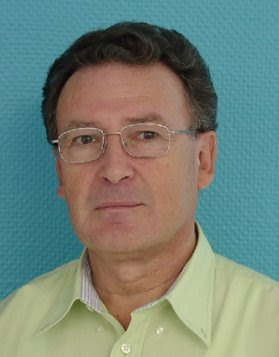
\includegraphics[width=.95\textwidth]{imgs/schwefel.jpg}
      \caption*{Hans-Paul Schwefel}
    \end{subfigure}%
    \begin{subfigure}{.3\textwidth}
      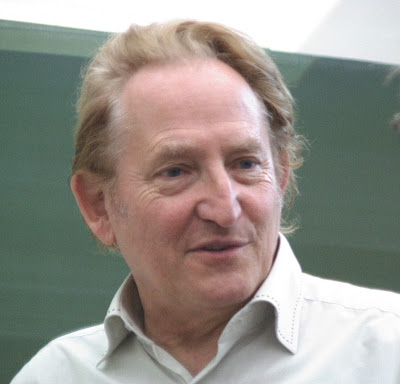
\includegraphics[width=.95\textwidth]{imgs/rechenberg.jpg}
      \caption*{Ingo Rechenberg}
    \end{subfigure}%
    \begin{subfigure}{.3\textwidth}
      
\includegraphics[width=.95\textwidth]{imgs/bienert.jpg}
      \caption*{Peter Bienert}
    \end{subfigure}
  \end{figure}

\end{frame}

\begin{frame}{Introducción}
  \begin{center}
    Experimento en túneles de viento
  \end{center}

  \begin{itemize}
  \item Técnicas clásicas
  \item Técnicas estocásticas
  \end{itemize}

  \begin{center}
    Nace la $(1 + 1) -$ ES
  \end{center}
\end{frame}

\begin{frame}{Siguientes éxitos}
  \begin{itemize}
  \item Bienert construye un robot para automatizar los cálculos
  \item Lichtfu{\ss} diseña una tubería
  \item Diseño de una tobera supersónica
  \end{itemize}
\end{frame}

\begin{frame}{Inconvenientes}
  \begin{itemize}
  \item Distribuciones binomiales
  \item Convergencia prematura a óptimos locales
  \end{itemize}

  \begin{center}
    Distribuciones normales
  \end{center}
\end{frame}

\begin{frame}{Mejoras de Rechenberg}
  \begin{itemize}
  \item $\frac{1}{5}$ \emph{th rule}
  \item Recombinación y autoadaptación: $(\mu + 1) -$ ES
  \end{itemize}
\end{frame}

\begin{frame}{Inconvenientes (II)}
  \begin{itemize}[<+- | alert@+>]
  \item Las $(\mu + 1) -$ ES tenían poca capacidad de autoadaptación.
  \item Surgen las $\left( \mu \ \overset{+}{,} \ \lambda \right)$
  \end{itemize}
\end{frame}

\begin{frame}{Críticas}
  \begin{itemize}
  \item Gran avance de los métodos numéricos en la década pasada
  \item Críticas a $\mu > 1$ y $\lambda > 1$
  \item Críticas a $(\mu, \lambda)$
  \end{itemize}
\end{frame}

\section{Programación genética}

\begin{frame}{Summary}

  Get the source of this theme and the demo presentation from

  \begin{center}\url{github.com/matze/mtheme}\end{center}

  The theme \emph{itself} is licensed under a
  \href{http://creativecommons.org/licenses/by-sa/4.0/}{Creative Commons
  Attribution-ShareAlike 4.0 International License}.

  \begin{center}\ccbysa\end{center}

\end{frame}

\begin{frame}[standout]
  Questions?
\end{frame}

\appendix

\begin{frame}[fragile]{Backup slides}
  Sometimes, it is useful to add slides at the end of your presentation to
  refer to during audience questions.

  The best way to do this is to include the \verb|appendixnumberbeamer|
  package in your preamble and call \verb|\appendix| before your backup slides.

  \themename will automatically turn off slide numbering and progress bars for
  slides in the appendix.
\end{frame}

\begin{frame}[allowframebreaks]{References}

  \bibliography{bibliography}
  \bibliographystyle{abbrv}

\end{frame}

\end{document}
